\documentclass[12pt]{article}

\usepackage{times}
\usepackage{amsmath, amssymb, multicol, graphicx}%pupr_paper,
\usepackage{listing}
\usepackage{verbatim}
\usepackage{booktabs}
\usepackage{float}
\usepackage[parfill]{parskip}
%\lstset{language=C++}
\usepackage[colorlinks = true, linkcolor = blue]{hyperref}

\setlength{\textwidth}{6.5in} \setlength{\textheight}{8.5in} \topmargin -0.3in \setlength{\rightmargin}{0.0in}
\setlength{\leftmargin}{.0in} \setlength{\oddsidemargin}{.0in} \labelwidth=1.2in \labelsep=0.1in
\parsep=0in
\parindent=0in
%\pagestyle{empty}
\setcounter{secnumdepth}{3}

\begin{document}
\begin{titlepage}
%\maketitle
 \centering
    \vspace*{15\baselineskip}
    \large
    \bfseries
    Software Project Management Plans  \\[3\baselineskip]
    \normalfont
     \vfill
    Emanuel Rivera Castro 53502 \\
    Yanilette Lopez Duprey 53990\\
    Joaquin Pockels Balaguer 54012\\[2\baselineskip]

    \textbf{\today} \\[2\baselineskip]
\end{titlepage}

\pagenumbering{roman}
\tableofcontents
\pagebreak
\listoftables
\pagebreak
\listoffigures
\clearpage\pagenumbering{arabic}

\section{Introduction}
 The purpose of this document named Software Project Management Plan is to establish in a clear form, the details and specifications of how this Project would be administrated. This document is going to facilitate the organization of the project, and it would guarantee that all the requirements are being fulfilled for the completion of the product.  This documents discuss the following topics:
\begin{itemize}
  \item Evolution of the SPMP
  \item Project Organization
  \item Managerial Process
  \item Technical Process
  \item Work Packages, Schedule and Budget
\end{itemize}
The SPMP is directed to:
\begin{enumerate}
  \item Clients - DARPA and Prof. Arturo Geigel
  \item Users - United States Armed Forces
  \item Developers - AIIP/S and people responsible for maintenance and making updates to the system.
\end{enumerate}

\subsection{Project Overview}
 Our project, is part of a proposal to Defense Advanced Research Projects Agency (DARPA). This proposal wants to decentralize control of unmanned vehicles and allows multiple operators to operate a single vehicle or formation of vehicles. This provides redundancy in the decision process and optimize the course of action to be followed. Our main focus is in the image segmentation/processing part. We receive images and classify them using a Probabilistic Neural Network (PNN) using 5 features: shape, color, location, normalized area and texture.

\subsection{Project Deliverables}
This subsection list all the items to be delivered to the customer, the delivery dates, delivery locations, and quantities to satisfy the terms of the project.
\begin{itemize}
  \item IEEE 1058 Software Project Management Plan\\
            Due Date: \\
            Quantity: 1\\
            Localization: L-310
  \item IEEE 830 Software Requirements Specification\\
            Due Date: \\
            Quantity: 1\\
            Localization: L-310
  \item IEEE 829 Software Test Document \\
            Due Date: \\
            Quantity: 1\\
            Localization: L-310

  \item IEEE 1016 Software Design Description\\
            Due Date:\\
            Quantity: 1\\
            Localization: L-310

  \item Image Segmentation/Processing Code\\
            Due Date:\\
            Quantity: 1\\
            Localization: L-310
\end{itemize}

\subsection{Evolution of the SPMP}
If any member of the group understands that the SPMP document needs to be updated for any reason, the member would have all the right to present a motion to express his point of view.  If the point of view is valid and is seconded by the two other members, the document would be updated. Each time a member finish a section he/she will give it to the other members for review.\\\\
The final version of the document will have the number 2.000. A change in the tenth position means that a new section was added, a change in the hundredth position means that a new subsection was added and a change in the thousandth position means that some subsection was modified.\\\\
Our main tool for updating this document is Github. Github is a repository where any member of the group can make changes without completely overwriting each other updates. As a second option, in case we experience any problems with Github, we will use dropbox to update this document.

\subsection{Reference Material}
This subsection provide a complete list of all the documents and other sources of information referenced in this document. Each document will be at least identified by title, author and date.\\\\
IEEE Documents:
\begin{itemize}
  \item IEEE Std 1058.1-1987  Software Project Management Plan\\
				Author: The Software Engineering Technical Committee of the Computer Society of the IEEE\\
                Date: Approved December 10, 1987\\
				PDF: ISBN 0-7381-0409-4, SS12138

  \item IEEE Std 829-1998  Software Test Documentation\\
				Author: The Software Engineering Technical Committee of the Computer Society of the IEEE\\
                Date: Approved 16 September 1998
				PDF:ISBN 0-7381-1444-8 SS94687

  \item IEEE Std 830-1998 Software Requirement Specification \\
				Author: The Software Engineering Technical Committee of the Computer Society of the IEEE \\
                Date: Approved 25 June 1998\\
				PDF: ISBN 0-7381-0332-2

  \item IEEE Std 1016-1998 Software Design Description\\
				Author: The Software Engineering Technical Committee of the Computer Society of the IEEE\\
                Date: Approved 23 September 1998\\
				PDF: ISBN 0-7381-1456-1 SS94688	
\end{itemize}

Papers:
\begin{itemize}
  \item Region-Based Image Retrieval Using Probabilistic Feature Relevance Learning\\
        Author: ByoungChul Ko, Jing Peng and Hyeran Byun
  \item Probabilistic Neural Networks SUpporting Multi-Class Relevance Feedback in Region-based Image Retrieval\\
        Author: ByoungChul Ko and Hyeran Byun\\
        Date: 2002
  \item FRIP: A Region-Based Image Retrieval Tool Using Automatic Image Segmentation and Stepwise Boolean AND Matching\\
        Author: ByoungChul Ko and Hyeran Byun\\
        Date: 2005
  \item A General Method for Unsupervised Segmentation of Images Using a Multiscale Approach\\
        Author: Alvin H. Kam and William J. Fitzgerald\\
        Date: 2000
\end{itemize}

Books:
\begin{itemize}
  \item Image Processing in C Second Edition\\
        Author: Dwayne Phillips
        Date: 2000
\end{itemize}

\subsection{Definitions and Acronyms}
This subsection shall define, or provide references to the definition of all terms and acronyms required to properly interpreted the SPMP.
\begin{table}[H]\centering
\begin{tabular}{|c|c|}
  \hline
  % after \\: \hline or \cline{col1-col2} \cline{col3-col4} ...
  Term & Definition \\
   \hline
   The Company & AIIPS \\
   \hline
   Software & Image Segmentation/Processing working code\\
   \hline
   Proposal & DARPA Proposal\\
   \hline
\end{tabular}
\caption{Definitions}
\end{table}

\begin{table}[H]\centering
\begin{tabular}{|c|c|}
  \hline
  % after \\: \hline or \cline{col1-col2} \cline{col3-col4} ...
  Term & Acronym \\
   \hline
   AIIPS & Artificial Intelligence and Image Processing/Segmentation   \\
    \hline
    PNN & Probabilistic Neural Network \\
    \hline
  Defense Advanced Research Projects Agency  & DARPA \\
   \hline
  Software Requirements Specification & SRS \\
   \hline
    Software Project Management Plan & SPMP \\
   \hline
     Software Test Document & STD \\
   \hline
     Software Design Description & SDD \\
   \hline
\end{tabular}
\caption{Acronyms}
\end{table}

\section{Project Organization}
This section of the SPMP specify the process model for the project, describe the project organizational boundaries and interfaces, and define individual responsibilities for the various project elements.\\\\
This section is divided in the following subsections:
\begin{itemize}
  \item Process Model
  \item Organizational Structure
  \item Organizational Boundaries and Interfaces
  \item Project Responsibilities
\end{itemize}

\subsection{Process Model}
The organization for the development of our software's documents (SRS, STD, SDD, SPMP and Code) will be paralleled and cascade. Each member will have a document assigned, this way the finish documentation can be completed by the due date the client specify. The process model also is cascaded because some sections in the documents might need other documents sections to be completed or defined.\\\\
Figure \ref{org_struct} shows the process model of the project. This cycle will repeat until all the documents are completed. This way we have a paralleled and cascaded model.

\begin{figure}[H]\centering
  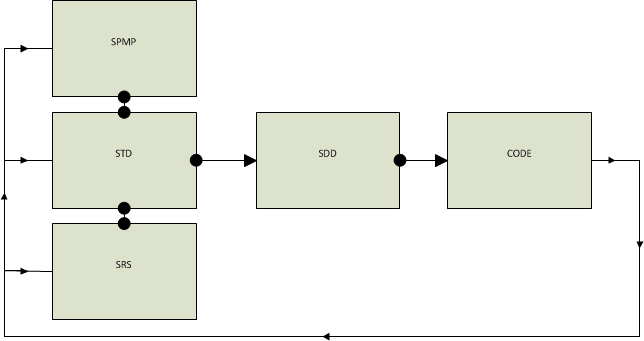
\includegraphics[width=6.0in]{block_diagram_Org_Struct}\\
  \caption{Block Diagram of the Process Model}\label{org_struct}
  \end{figure}

\subsection{Organizational Structure}
AIIPS consists of 3 members:
\begin{itemize}
  \item Emanuel Rivera Castro - Team Leader / SPMP
  \item Yanilette Lopez Duprey - Writes the weekly reports / STD
  \item Joaquin Pockels Balaguer - Programmer / SRS, SDD
\end{itemize}

Decisions within the Company are handled through voting. The changes must be discussed by the group, after which a debate will take place to find the advantages and disadvantages. Finally, the group will vote and majority decided whether the change will take place. Each meeting will be documented in the weekly report.\\\\
Communication between group members will consist of phone calls, text messages and meetings. Generally, meetings take place every Wednesday at 1:30pm with additional meetings taking place during whenever the group decides is necessary.

\subsection{Organizational Boundaries and Interfaces}
As section 1 of this documents says our main purpose/objective in the project is to implement the image segmentation/processing of the DARPA proposal. In a real life situation we will be receiving images from an external agent, segment and classify those images and send back to the agent the classification. For the testing we will be using a set of images. Other companies/organizations will take care of the other components of this proposal.\\\\
Figure \ref{boundaries} shows the relevant parts for this project of the DARPA proposal. We don't care who or how the other agents do their work, our only concern is to have images as input to our Software.

\begin{figure}[H]\centering
  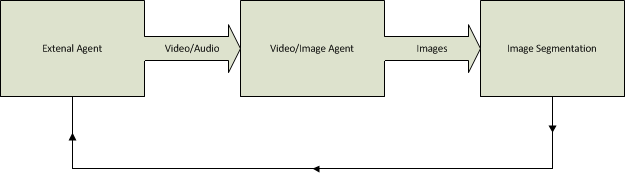
\includegraphics[width=6.0in]{boundaries}\\
  \caption{Block Diagram of the Boundaries of our Project}\label{boundaries}
  \end{figure}

\subsection{Project Responsibilities}
It is important to note that there will be at least one manager per document. The manager(s) of the document will be listed with the documents type also indicating the other member(s) that were assigned to work under that document.Tables \ref{RespMem}-\ref{RespSPMP} shows the responsibilities of each member.
%In addition it is important to understand that there are more responsibilities unrelated to the documents that need to be done. These responsibilities are more related the project status of which each member should have often known as job titles. In our case a member working on this project could have more than one title and these titles imply their responsibilities within the current project.

\begin{table}[H]\centering
\begin{tabular}{|c|c|c|}
  \hline
  % after \\: \hline or \cline{col1-col2} \cline{col3-col4} ...
  Document & Project Manager(s) & Assigned Member(s) \\
   \hline
   AIIPS SRS & Joaquin Pockels & Emanuel Rivera, Yanilette Lopez \\
   \hline
   AIIPS SDD & Joaquin Pockels & Emanuel Rivera, Yanilette Lopez\\
   \hline
   AIIPS STD & Yanilette Lopez & Emanuel Rivera, Joaquin Lopez  \\
   \hline
   AIIPS SPMP & Emanuel Rivera & Joaquin Lopez, Yanilette Lopez \\
   \hline
   AIIPS Software & Joaquin Pockels & Emanuel Rivera, Yanilette Lopez \\
   \hline
\end{tabular}
\caption{Main Responsibilities for each member}
\label{RespMem}
\end{table}

\begin{table}[H]\centering
\begin{tabular}{|c|c|c|}
  \hline
  \multicolumn{3}{|c|}{SRS} \\
  \hline
  % after \\: \hline or \cline{col1-col2} \cline{col3-col4} ...
  Title & Section(s) & Member(s) \\
   \hline
    &  &  \\
   \hline
\end{tabular}
\caption{Shows who works in each section of the SRS}
\label{RespSRS}
\end{table}

\begin{table}[H]\centering
\begin{tabular}{|c|c|c|}
  \hline
  \multicolumn{3}{|c|}{SDD} \\
  \hline
  % after \\: \hline or \cline{col1-col2} \cline{col3-col4} ...
  Title & Section(s) & Member(s) \\
   \hline
    &  &  \\
   \hline
\end{tabular}
\caption{Shows who works in each section of the SDD}
\label{RespSDD}
\end{table}

\begin{table}[H]\centering
\begin{tabular}{|c|c|c|}
  \hline
  \multicolumn{3}{|c|}{STD} \\
  \hline
  % after \\: \hline or \cline{col1-col2} \cline{col3-col4} ...
  Title & Section(s) & Member(s) \\
   \hline
    &  &  \\
   \hline
\end{tabular}
\caption{Shows who works in each section of the STD}
\label{RespSTD}
\end{table}

\begin{table}[H]\centering
\begin{tabular}{|c|c|c|}
  \hline
  \multicolumn{3}{|c|}{SPMP} \\
  \hline
  % after \\: \hline or \cline{col1-col2} \cline{col3-col4} ...
  Title & Section(s) & Member(s) \\
   \hline
   Introduction, Project Organization, Managerial Process & 1-3  & Emanuel Rivera \\
   \hline
\end{tabular}
\caption{Shows who works in each section of the SPMP}
\label{RespSPMP}
\end{table}

\section{Managerial Processes}
This section shall specify management objectives and priorities; project assumptions, dependencies, and constraints; risk management techniques; monitoring and controlling mechanisms to be used; and the staffing plan.\\\\
This section is divided in the following subsections:
\begin{itemize}
  \item Management objectives and priorities
  \item Project assumptions, dependencies and constraints
  \item Risk management techniques (3.3)
  \item Monitoring and controlling mechanisms to be used
  \item Staffing Plan
\end{itemize}

\subsection{Management Objectives and Priorities}
This section contains first, the philosophy, goals and priorities on management activities for the project. Also it will specify the format used for reporting and the expected frequency of reports during the project, priorities among requirements on the project and the project’s schedule and budget.

\subsubsection{Philosophy}
The philosophy adopted for the management of activities is divide and conquer. The group will usually meet either physically or via other means of communication such as internet conference calls using Skype or phone calls. Afterwards the activity is discussed by the members and decomposed into essential parts or tasks required for the activity completion which are then assigned to a corresponding project member in order for a swift completion of the activity.

\subsubsection{Goals}
The goals are simply to be able to fulfill the objectives of this stage of the Proposal and writing each document as fast as possible so we can have feedback from our client and proceed to the next activity. The swifter the completion of an activity the more time the project team will have to review and audit the activity with the purpose of obtaining desired quality control on an activity.

\subsubsection{Priorities}
The priorities on an activity may vary on the difficulty of completion of said activity, also priorities can be viewed as the time and project resources allocated on the completion of an activity, the greater time and project resources allocated to an activity, the higher the priority of the activity. \\\\
	The order established for the main activity priorities are the following:

\begin{enumerate}
  \item Doumenting the plan (SPMP) and the requirements (SRS) of the Project.
  \item Documenting the design (SDD) and testing methods (STD) of the Project.
  \item Work on AIIPS Software.
  \item Meet with our client for feedback.
\end{enumerate}

\subsubsection{Project Budget Priorities}
The priority on the project budget allocation was the following:
\begin{itemize}
  \item Computers for the project staff
  \item Required hardware and software for the project’s completion
  \item Papers necessary for a better understanding of the process/steps to complete this Project.
\end{itemize}

\subsubsection{Risk Management Procedures}
In the event that a risk or problematic situation occurs during the development of the project, an emergency staff meeting will take place in order to address the problem or situation. On these meeting it’s imperative to hear each of the staff member’s opinion and possible solutions on the matter. Afterwards the project staff will proceed to make a democratic vote election to determinate the course of action to be taken based on the proposed or accepted solutions to the given risk or problem.

\subsubsection{Software Acquisition Statement Management}
The proper format to deliver a statement which states the intention of acquiring, modifying or using existing software should follow the following procedure:

\begin{itemize}
  \item	Mention the Software in question during a staff meeting.
  \item State the reasons why the existing software is needed.
  \item Mention and justify the amount of software licenses needed
  \item Afterwards the staff in democratic vote will decide to acquire the software or not.
\end{itemize}

\subsection{Assumptions, Dependencies and Constraints}
This section will contain information regarding the necessary assumptions on which the project is based, external events the project is dependent upon in order to complete itself and constraints on which the project will be conducted.

\subsubsection{Assumptions}
The Assumptions for this project are the following:

\begin{enumerate}
  \item The client already had design a complete robot/agent that captures video and audio.
  \item The client already had design the communication protocol to send the image and video.
  \item The client already had design the process/algorithm to take the video and divide it in frames/images.
  \item The staff assigned to system maintenance have knowledge of a PNN.
\end{enumerate}
\subsubsection{Dependencies}
Most of the dependencies of external events the project will be dependent upon will be due the completion of the project documentations. For example SDD and STD documents will be dependent on the completion of the SRS and SPMP documentations in order for their completion to be successful. Other dependencies would be the feedback from our client that may change/alter the code and/or documents.
\subsubsection{Constraints}
The following were the constraints of the project:
\begin{enumerate}
  \item A deadline of 3 months for the documentation and a working code.
  \item Project documents must comply with IEEE  software documentation format
  \item All the requirements mentioned in the SRS.
\end{enumerate}

\subsection{Risk Management}
This subsection identify and assess the risk factors associated with the project. It prescribe mechanisms for tracking the various risk factors and implementing contingency plans.

\begin{itemize}
  \item \textbf{Risk regarding contract:}\\\\
  Examples would be not complying with the established deadline by the costumer. Another example would be violations of the contract terms from either end of the contract. These are the most common situations that may occur during project development.
  \item \textbf{Risk’s regarding technology related on the project:}\\\\
      An example would be damage received to project data resulting in it’s loss. Other situations that could occur are damage or theft of computer equipment or other materials.
  \item \textbf{Risk’s regarding size and complexity of the product:}\\\\
      An example of these risks would be that requirements and constraints of the project may require strong attention to detail and extensive documentation that may require more time that the established deadline. Another example could be disagreement on the design approach to solve a particular problem regarding the project’s development which may result on delaying progress on the project’s development.
  \item \textbf{Risks regarding personnel acquisition and retention:}\\\\
      Examples of these risks would be that a member may not have the required skill and expertise in order to perform assigned tasks which would hinder greatly the project’s development. Another example would be that a project staff member doesn’t complete the assigned task or that the completed task does not meet the expected standards. Another possible example would be the inconsistency of a project member to show up on meetings or having lack of communication with other project staff members resulting in a hindrance to the project’s development for not being in par with the progress of the project’s development.
  \item \textbf{Risks regarding consumer acceptance of the product:}\\\\
      Examples would be the customer may not express the desired resulting product correctly and mid development forces the staff member to redo most of the currently developed product on the project. Another example would be additional requests from the customer that may require drastic changes on the currently developed product.  Finally a risk example would be that the final product doesn’t comply with the requirements and constraints given by the client resulting in customer’s dissatisfaction, termination of the contract, revenue loss, loss of the company’s reputation, company bankruptcy and other undesired situations.
\end{itemize}

\subsection{Monitoring and Controlling Mechanisms}
This section would briefly contain information about flow of information and controlling and auditing mechanisms as well as tools used in order to aid this task. These all apply to all the work packages regarding this project. 
\begin{itemize}
  \item \textbf{Flow of Information}\\\\
  Most of the information regarding the project is being kept digitally in documents stored as data on computers. Also information may flow via personal means or telecommunication tools such as cell phones, text messages, Skype conference calls , Dropbox  and GitHub Repository.
  \item \textbf{Review and Audit Mechanisms}\\\\
  The member assigned to each document will open and review the work done on the documentation using Dropbox or GitHub. We are going to use Latex to edit and modify each document. If changes are necessary to a current work done in order to comply with the requirements, constraints and IEEE standards, the editor will notify the staff member responsible of the work in question the necessary changes via any of the mentioned tools in Flow of Information. If necessary and the editor in chief has the required skill and preparation, he may do the corresponding modifications to the work under review and audit.
  \item The tools used for Monitoring and controlling mechanisms are the following:
      \begin{enumerate}
        \item Dropbox
        \item GitHub
        \item WinEdt 7(Latex) 
        \item Emacs (for Latex)
      \end{enumerate}
\end{itemize}

\subsection{Staffing Plan}
The Project can be developed with a small group consisting of five (3) members. They, however, have to meet the following requirements:
\begin{enumerate}
  \item Experience with C.
  \item Able to start August 13, 2012.
  \item Able to work until November.
  \item Must have time to attend meetings.
  \item Bachelor degree on computer science and or Computer Engineering
  \item Willing to work on flexible schedules
  \item No previous field experience is required
  \item Capable of following instructions
  \item Be able to work with other team members
  \item Basic knowledge of IEEE standard software documentation.

\end{enumerate}



\end{document}
